\documentclass{beamer}
\usetheme{Warsaw}
% \usetheme{metropolis}

\usepackage[backend=biber, style=authoryear, backref=true, hyperref=true]{biblatex}
\addbibresource{biblio.bib}

\usepackage{version}
\usepackage[utf8]{inputenc}
% \usepackage[french]{babel}
\usepackage[T1]{fontenc}
\usepackage{amsmath,mathtools}
\usepackage{amssymb}
\usepackage{amsthm}
\usepackage{bbm}
\usepackage{relsize}
\usepackage{multirow}
\usepackage{hyperref}
\hypersetup{colorlinks=true, citecolor=green, linkcolor=blue, urlcolor=blue}
\usepackage{color}
\usepackage{caption}
\captionsetup[figure]{labelformat=empty}

\usepackage{tikz}
% \usetikzlibrary{shapes,positioning,arrows,shapes.arrows, decorations.markings,arrows.meta,decorations.pathreplacing}
\usetikzlibrary{backgrounds}

\setbeamertemplate{headline}{}

% \addtobeamertemplate{block begin}{%
%   \setlength{\textwidth}{1.05\textwidth}%
% }{}

\newcommand{\gw}{\text{GW}}
\newcommand{\ot}{\text{OT}}
\newcommand{\coot}{\text{COOT}}

\newcommand{\ugw}{\text{UGW}}
\newcommand{\agw}{\text{AGW}}
\newcommand{\uot}{\text{UOT}}
\newcommand{\ucoot}{\text{UCOOT}}
\newcommand{\fgw}{\text{FGW}}
\newcommand{\fugw}{\text{FUGW}}
\newcommand{\kl}{\text{KL}}

\newcommand{\cX}{\mathcal X}
\newcommand{\cY}{\mathcal Y}
\newcommand{\cM}{\mathcal M}
\newcommand{\bbR}{\mathbb R}
\newcommand{\rmd}{\mathrm{d}}
\newcommand{\bX}{\textbf{X}}
\newcommand{\bY}{\textbf{Y}}

\newcommand{\pis}{{\color{blue}{\pi^s}}}
\newcommand{\pif}{{\color{red}{\pi^f}}}

\newcommand{\mfsrc}{{\color{red}{\mu_1^f}}}
\newcommand{\mftg}{{\color{red}{\mu_2^f}}}
\newcommand{\mssrc}{{\color{blue}{\mu_1^s}}}
\newcommand{\mstg}{{\color{blue}{\mu_2^s}}}

\setlength{\leftmargini}{0.2cm}
\setlength{\leftmarginii}{0.1cm}

\newtheorem{proposition}{Proposition}[section]
\newtheorem{assumption}{Assumption}

%%%%%%%%%%%%%%%%%%%%%%%%%%%%%%
%%%%%%%%%%%%%%%%%%%%%%%%%%%%%%

%Information to be included in the title page:
\title[PhD Defense]{Optimal Transport for Transfer Learning Across Spaces}

\author[]{Quang Huy Tran \break \tiny{Under the supervision of Nicolas Courty, Karim Lounici and Rémi Flamary}}

\institute[] % (optional)
{
  \inst{1}%
  Institut de Recherche en Informatique et Systèmes Aléatoires - IRISA \\
  Université Bretagne Sud
  \and
  \inst{2}%
  Centre de Mathématiques Appliquées - CMAP \\
  Ecole Polytechnique
}

\date[] % (optional)
{PhD Defense, 16 May 2024, Palaiseau}

\begin{document}

\frame{\titlepage}

\AtBeginSection[]
{
  \begin{frame}
    \frametitle{Table of Contents}
    \tableofcontents[currentsection]
  \end{frame}
}

%%%%%%%%%%%%%%%%%%%%%%%%%%%%%%%%%%%%%
\section{Introduction}
%%%%%%%%%%%%%%%%%%%%%%%%%%%%%%%%%%%%%
\begin{frame}

\end{frame}

%%%%%%%%%%%%%%%%%%%%%%%%%%%%%%%%%%%%%
\begin{frame}{Across-space comparison}
  \tiny
  \begin{block}{Gromov-Wasserstein distance \parencite{Memoli07,Memoli11}}
  Given two metric-measure spaces $\cX_1 = (X_1, \mu_1, d_1)$ and
  $\cX_2 = (X_2, \mu_2, d_2)$,
  \begin{align*}
    \gw_p^p(\cX_1, \cX_2) = \inf_{\pi \in U(\mu_1, \mu_2)}
    \iint \left| d_1(x_1, x_1') - d_2(x_2, x_2') \right|^p
    \rmd\pi(x_1, x_2) \rmd\pi(x_1', x_2')
  \end{align*}
\end{block}

\begin{minipage}[t]{0.58\linewidth}
\begin{enumerate}
  \item Metric properties + Isometries.
  \item Not the only way to compare incomparable spaces

  $\Rightarrow$ Gromov-Hausdorff distance.
  \item Add something more
\end{enumerate}
\end{minipage}%
\hfill%
\hspace{-6cm}
\begin{minipage}[t]{0.5\linewidth}
  \vspace{-0.2cm}
\begin{figure}
  \centering
  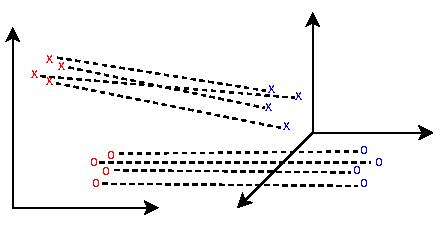
\includegraphics[width=1.2\linewidth, keepaspectratio=true]{OT_new/gw.pdf}
\end{figure}
\end{minipage}

\end{frame}

%%%%%%%%%%%%%%%%%%%%%%%%%%%%%%%%%%%%%
\begin{frame}{Extensions}
  \tiny
  \begin{enumerate}
    \item Measure networks \parencite{Chowdhury19}.
    \item Sliced-GW \parencite{Vayer19a},
    \item Low-rank GW \parencite{Meyer21b}.
  \end{enumerate}
  \begin{minipage}[t]{0.5\linewidth}
    \begin{itemize}
      \item Our focus
      \begin{enumerate}
        \item Bilinear relaxation.
        \item Marginal relaxation.
        \item Shared space.
      \end{enumerate}
    \end{itemize}
    \end{minipage}%
    \hfill%
    \hspace{-6cm}
    \begin{minipage}[t]{0.8\linewidth}
      \vspace{-2cm}
    \begin{figure}
      \centering
      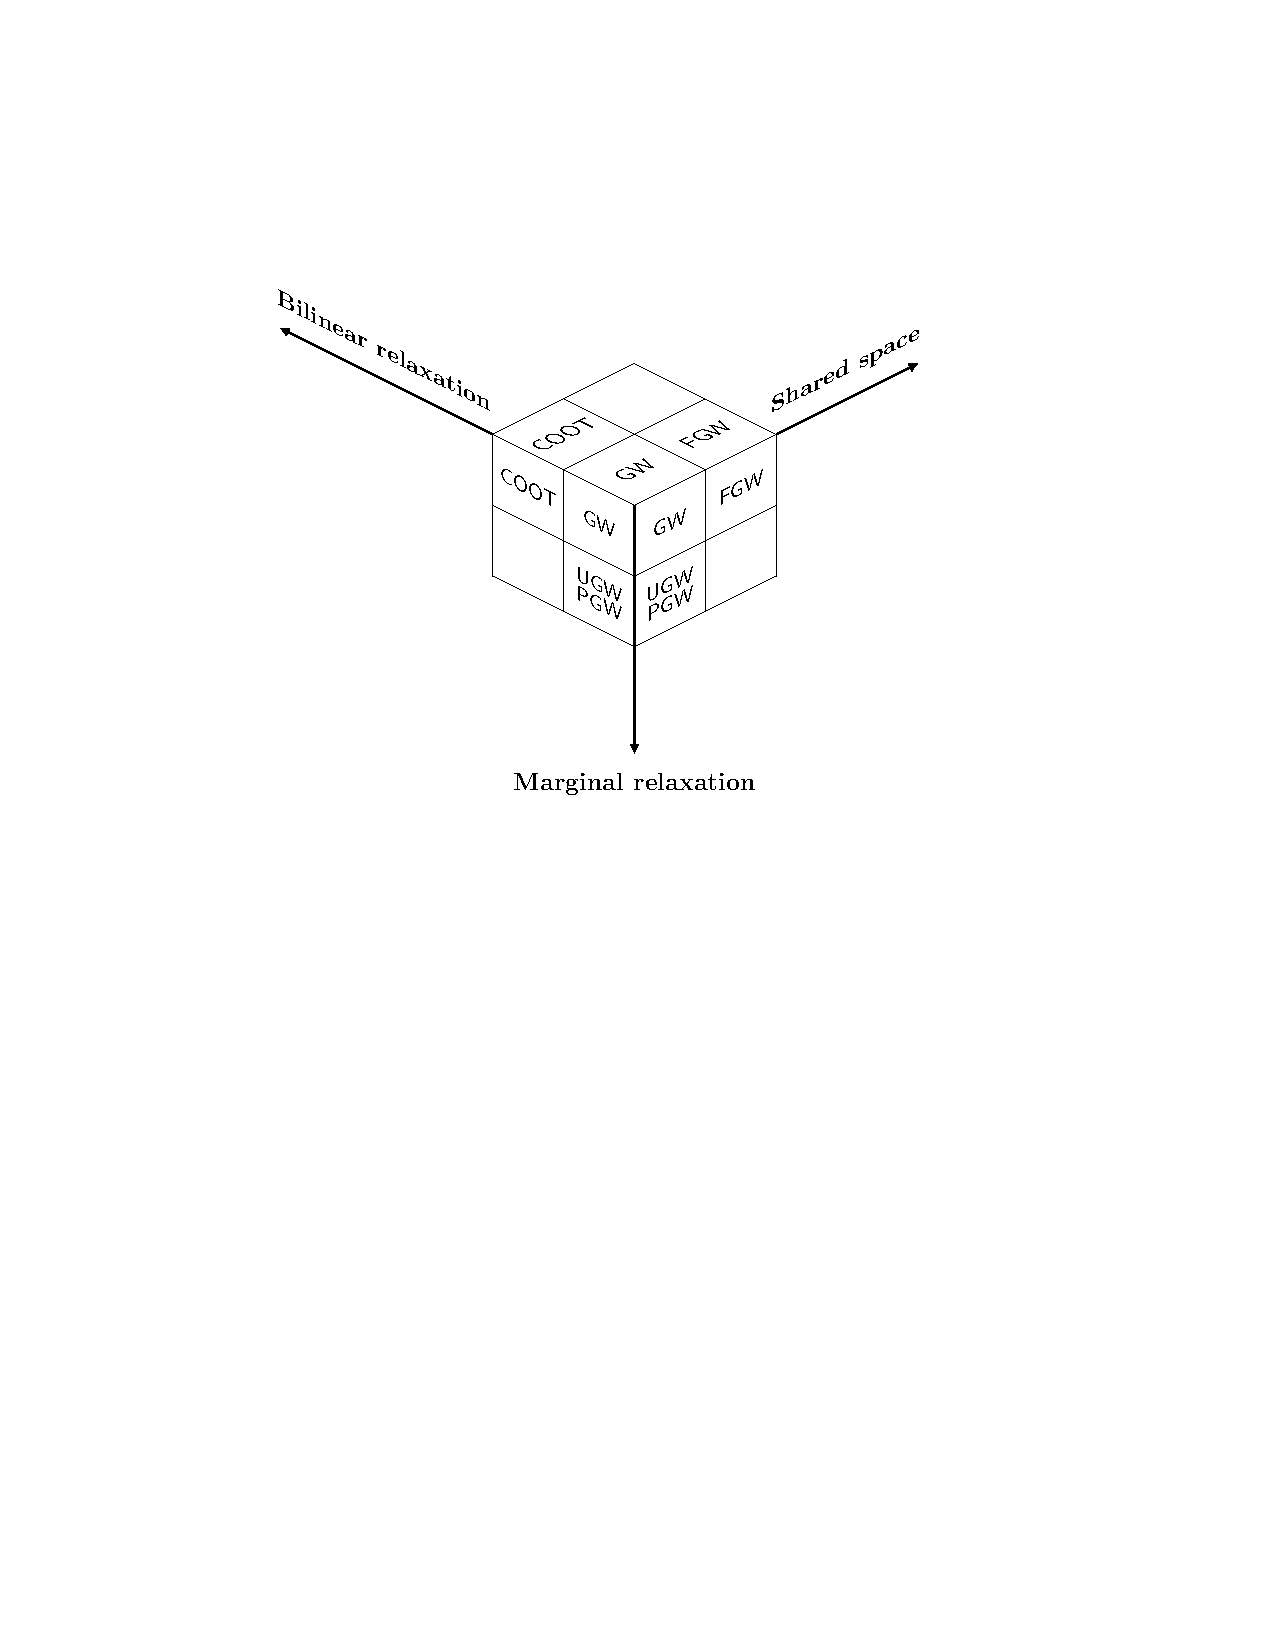
\includegraphics[width=1.2\linewidth, keepaspectratio=true]{OT_new/cube_extension.pdf}
    \end{figure}
    \end{minipage}
\end{frame}


%%%%%%%%%%%%%%%%%%%%%%%%%%%%%%%%%%%%%
\begin{frame}{Unbalanced Gromov-Wasserstein}
  \vspace{-0.2cm}
  \tiny
  \begin{definition}[Unbalanced GW \parencite{Sejourne20}]
    Given two compact metric-measure spaces $\cX_1 = (X_1, \mu_1, d_1),
    \cX_2 = (X_2, \mu_2, d_2)$ and a Csiszár divergence $D_{\varphi}$,
    \begin{align*}
      \ugw_p^p(\cX_1, \cX_2) = \inf_{\pi \in \cM^+(X_1 \times X_2)} L_{\ugw}(\pi),
    \end{align*}
    \vspace{-0.3cm}
    where
    \begin{align*}
      L_{\ugw}(\pi) &= \iint \left| d_1(x_1, x_2) - d_2(y_1, y_2) \right|^p
      \rmd\pi(x_1, y_1) \rmd\pi(x_2, y_2) \\
      &+ \rho_1 D_{\varphi}(\pi_{\# 1} \otimes \pi_{\# 1} | \mu_1 \otimes \mu_1)
      + \rho_2 D_{\varphi}(\pi_{\# 2} \otimes \pi_{\# 2} | \mu_2 \otimes \mu_2).
    \end{align*}
  \end{definition}

  \begin{minipage}[t]{0.6\linewidth}
  \begin{itemize}
    \item In practice: $D_{\varphi} = \text{Kullback-Leibler div}$.
    \item Characterizing isometries.
    \item Practical robustness to outliers.
    \item Approx. with/without entropic reg.
  \end{itemize}
  \end{minipage}%
  \hfill%
  \hspace{-6cm}
  \begin{minipage}[t]{0.45\linewidth}
    \vspace{-0.5cm}
  \begin{figure}
    \centering
    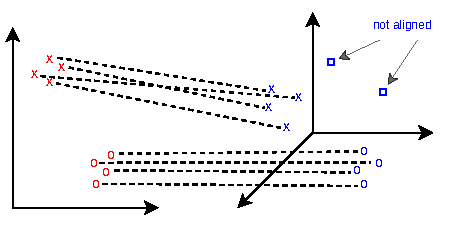
\includegraphics[width=1.2\linewidth, keepaspectratio=true]{OT_new/ugw.pdf}
  \end{figure}
  \end{minipage}

\end{frame}

%%%%%%%%%%%%%%%%%%%%%%%%%%%%%%%%%%%%%
\begin{frame}{Fused Gromov-Wasserstein}
  \tiny
  \begin{definition}[Fused GW \parencite{Vayer19b}]
    Consider two attributed graphs $\cX_1 = (D_1, F_1, \mu_1)$ and
    $\cX_2 = (D_2, F_2, \mu_2)$,
    where $D_k \in \bbR^{n_k \times n_k}, F_k \in \bbR^{n_k \times d}$
    and $\mu_k \in \Delta_{n_k}$. For $\alpha \in [0, 1]$,
    \begin{align*}
      \fgw_p^p(\cX_1, \cX_2) = \inf_{\pi \in U(\mu_1, \mu_2)} L_{FGW}(\pi),
    \end{align*}
    \vspace{-0.3cm}
    where
    \begin{align*}
      L_{FGW}(\pi) = (1 - \alpha)
      \sum_{{\color{blue}{i}},{\color{blue}{j}},{\color{red}{k}},{\color{red}{l}}}
      |(D_1)_{{\color{blue}{i}} {\color{red}{k}}} - (D_2)_{{\color{blue}{j}}{\color{red}{l}}}|^p {\color{blue}{\pi_{ij}}} {\color{red}{\pi_{kl}}}
      + \alpha \sum_{ij} ||(F_1)_i - (F_2)_j||^q \pi_{ij}.
    \end{align*}
  \end{definition}

  \begin{minipage}[t]{0.6\linewidth}
    \begin{itemize}
      \item Interpolation between GW and Wasserstein distances.
      \item Feature-preserving isometries.
    \end{itemize}
    \end{minipage}%
    \hfill%
    \hspace{-6cm}
    \begin{minipage}[t]{0.5\linewidth}
      \vspace{-0.cm}
    \begin{figure}
      \centering
      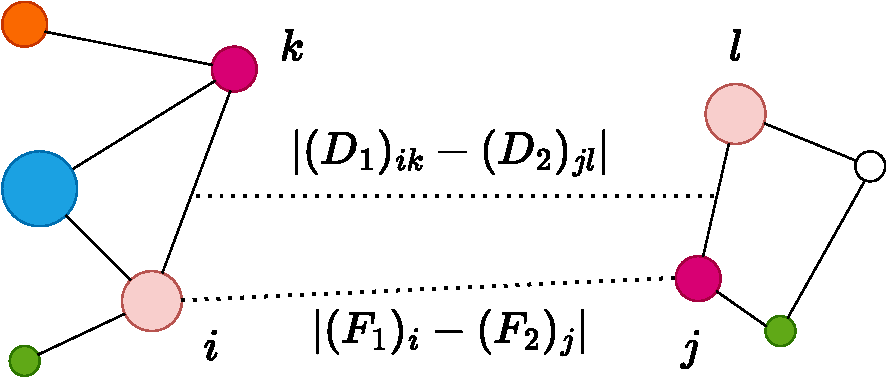
\includegraphics[width=\linewidth, keepaspectratio=true]{OT_new/fgw.pdf}
      % \caption*{\tiny{Inspired by \parencite{Vayer19b}}}
    \end{figure}
    \end{minipage}

\end{frame}

%%%%%%%%%%%%%%%%%%%%%%%%%%%%%%%%%%%%%
\begin{frame}{Co-Optimal Transport}
\tiny
\begin{definition}[Discrete COOT \parencite{Redko20}]
Given two weighted matrices $\cX_1 = (X_1, \mssrc, \mfsrc)$
and $\cX_2 = (X_2, \mstg, \mftg)$, where
$X_k \in \bbR^{n_k \times d_k}$ and histograms
${\color{blue}{\mu^s_k \in \Delta_{n_k}}}, {\color{red}{\mu^f_k \in \Delta_{d_k}}}$
\begin{align*}
  \coot_p^p(\cX_1, \cX_2) =
  \min_{\substack{\pis \in U(\mssrc,\mstg) \\ \pif \in U(\mfsrc,\mftg)}}
  \sum_{{\color{blue}{i}},{\color{blue}{j}},{\color{red}{k}},{\color{red}{l}}}
  |(X_1)_{{\color{blue}{i}} {\color{red}{k}}} - (X_2)_{{\color{blue}{j}}{\color{red}{l}}}|^p {\color{blue}{\pi^s_{ij}}} {\color{red}{\pi^f_{kl}}}
\end{align*}
\end{definition}

\begin{minipage}[t]{0.6\linewidth}
  \begin{itemize}
    \item Comparing \underline{arbitrary-size} matrices.
    \item Meaningful {\color{red}{feature}} coupling $\pif$.
    \item Metric properties.
    \item Connection with GW distance.
    \item Continuous extension \parencite{Chowdhury21b}.
  \end{itemize}
  \end{minipage}%
  \hfill%
  \hspace{-6cm}
  \begin{minipage}[t]{0.55\linewidth}
    \vspace{0cm}
  \begin{figure}
    \centering
    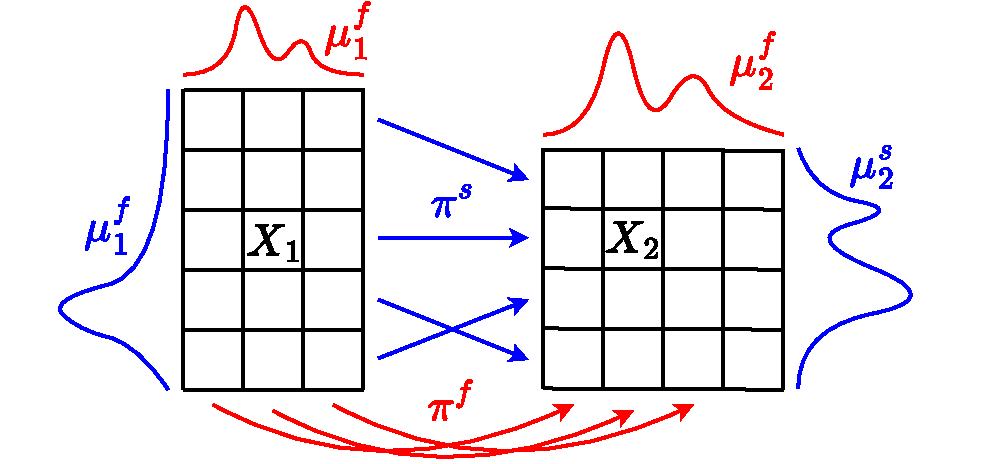
\includegraphics[width=1.2\linewidth, keepaspectratio=true]{OT_new/coot_matrix_ot.pdf}
  \end{figure}
  \end{minipage}
\end{frame}
%%%%%%%%%%%%%%%%%%%%%%%%%%%%%%%%%%%%%

\begin{frame}{Summary of contributions}
  \tiny
  Publication: \underline{Unbalanced Co-Optimal Transport}.
  \textbf{QHT}, Hicham Janati, Nicolas Courty, Rémi Flamary, Ievgen Redko, Pinar Demetci and Ritambhara Singh. \textit{AAAI Conference on Artificial Intelligence}, 2023.
  \vspace{-2.5cm}
  \begin{figure}
    \centering
    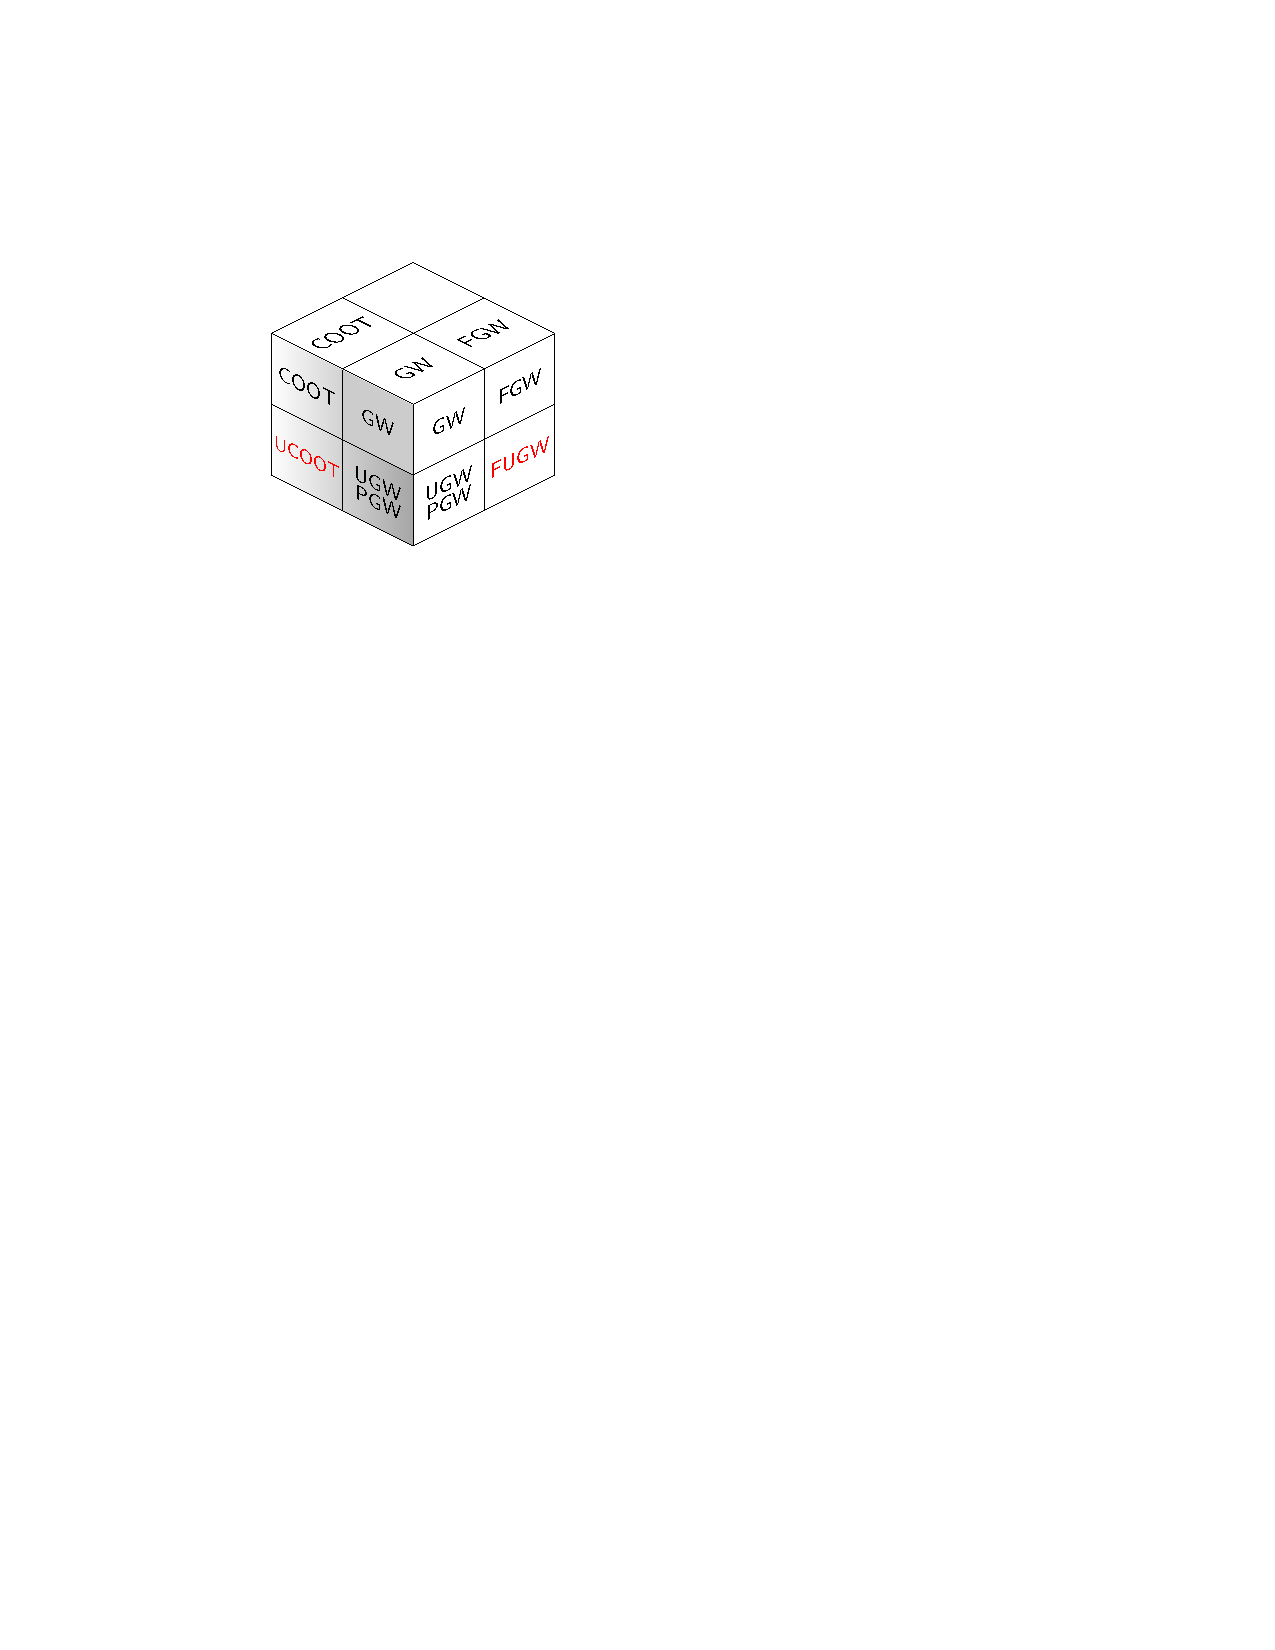
\includegraphics[width=1.1\linewidth, keepaspectratio=true]{OT_new/cube_ucoot.pdf}
  \end{figure}
\end{frame}

\begin{frame}{Summary of contributions}
  \vspace{-1cm}
  \begin{figure}
    \centering
    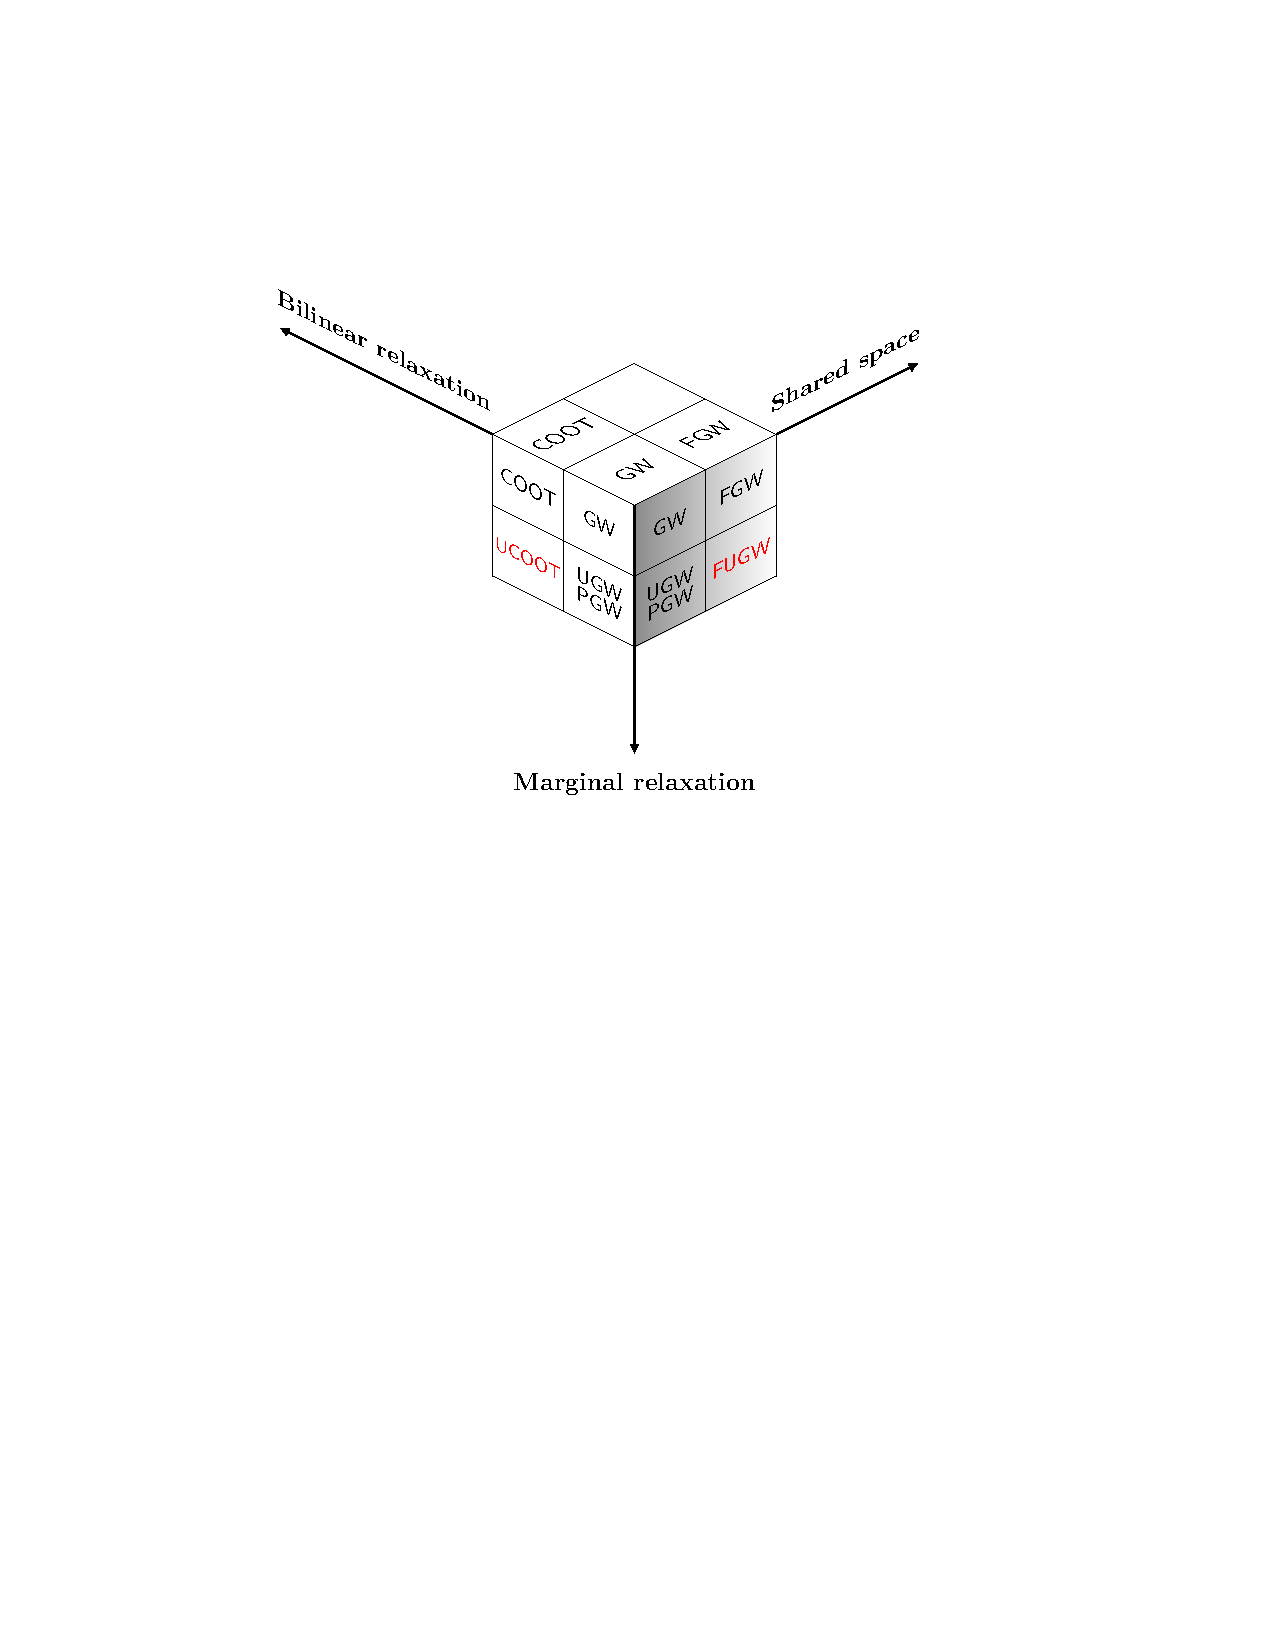
\includegraphics[width=1.1\linewidth, keepaspectratio=true]{OT_new/cube_fugw.pdf}
  \end{figure}
\end{frame}

\begin{frame}{Summary of contributions}
  \tiny
  Publication:
  \vspace{-2cm}
  \begin{figure}
    \centering
    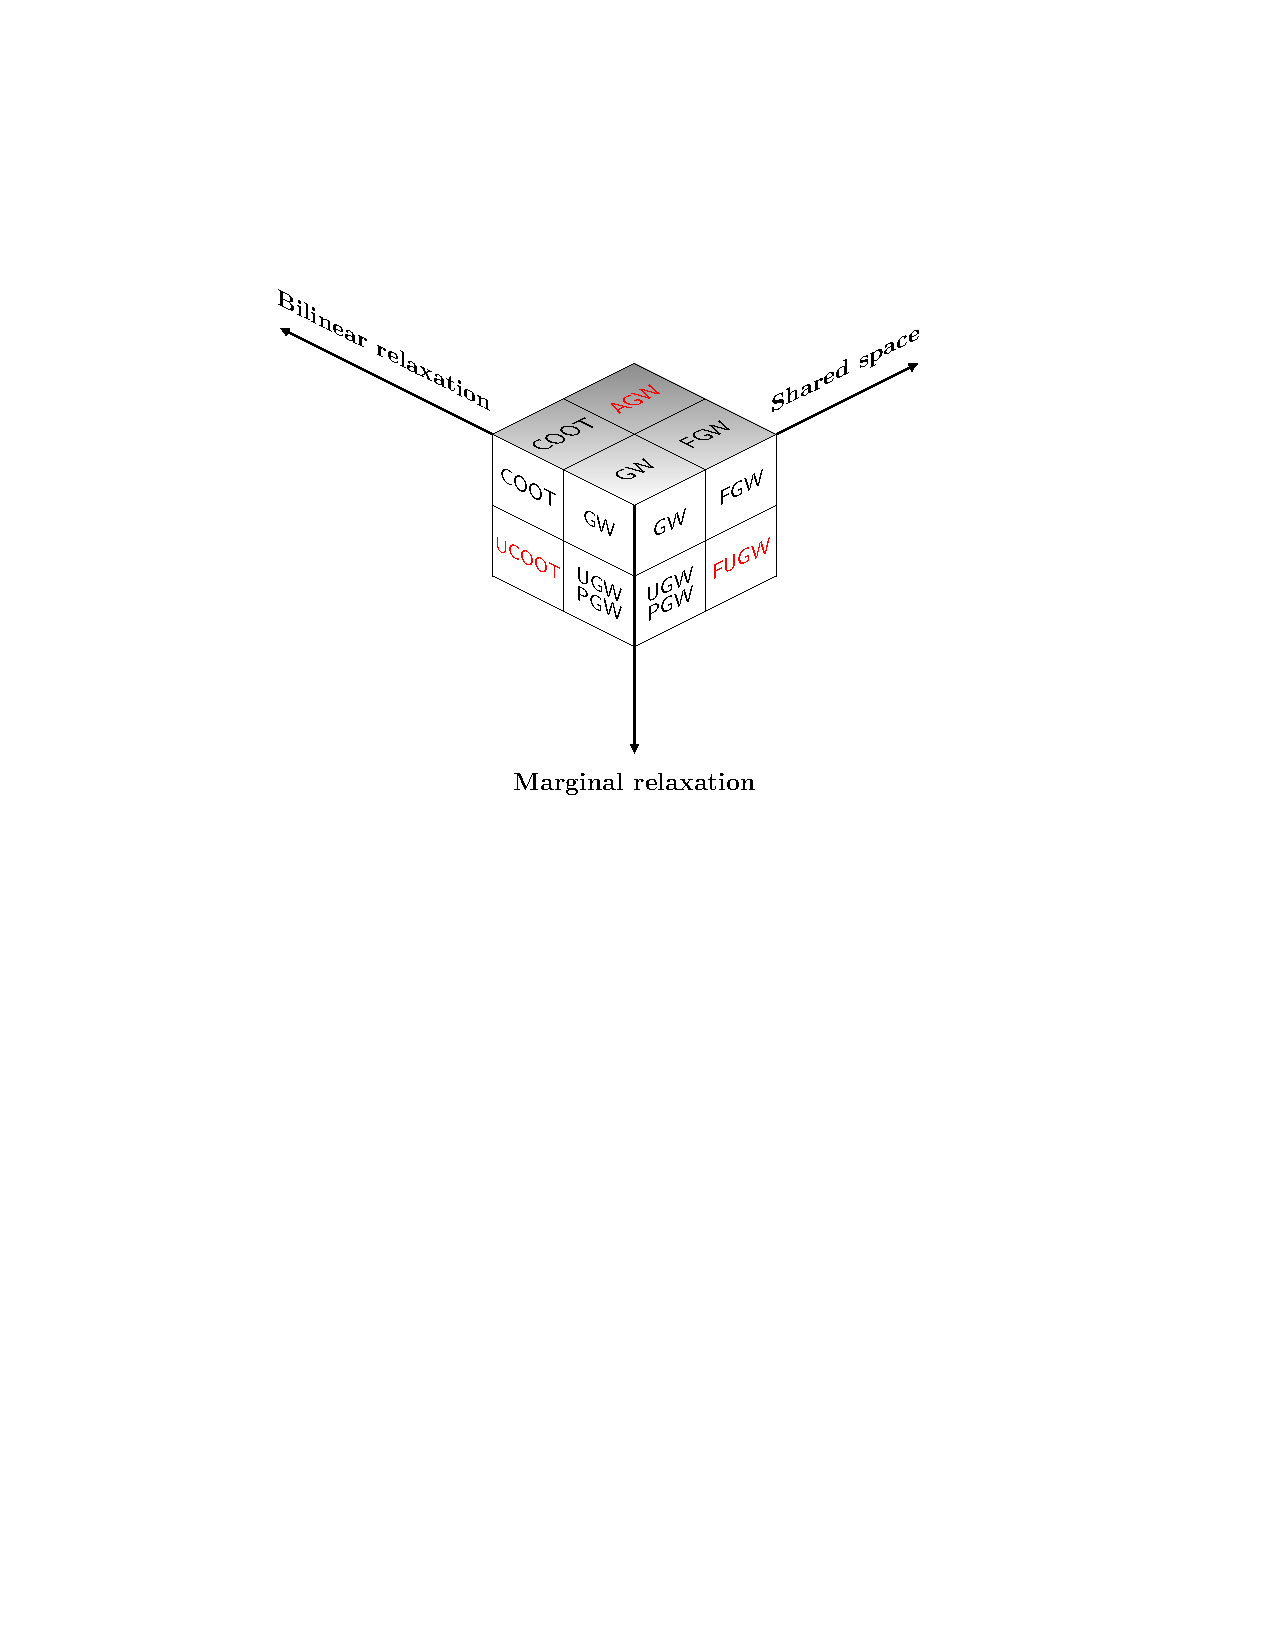
\includegraphics[width=1.1\linewidth, keepaspectratio=true]{OT_new/cube_agw.pdf}
  \end{figure}
\end{frame}

%%%%%%%%%%%%%%%%%%%%%%%%%%%%%%%%%%%%%%%%%%%%%%%%%%%%%%%%%%%%%%%%%%%%%%
%%%%%%%%%%%%%%%%%%%%%%%%%%%%%%%%%%%%%%%%%%%%%%%%%%%%%%%%%%%%%%%%%%%%%%
%%%%%%%%%%%%%%%%%%%%%%%%%%%%%%%%%%%%%%%%%%%%%%%%%%%%%%%%%%%%%%%%%%%%%%
%%%% Contribution on UCOOT
\section{Unbalanced CO-Optimal Transport}

%%%%%%%%%%%%%%%%%%%%%%%%%%%%%%%%%%%%
\begin{frame}{Motivation (1)}
\tiny
\begin{figure}
  \centering
  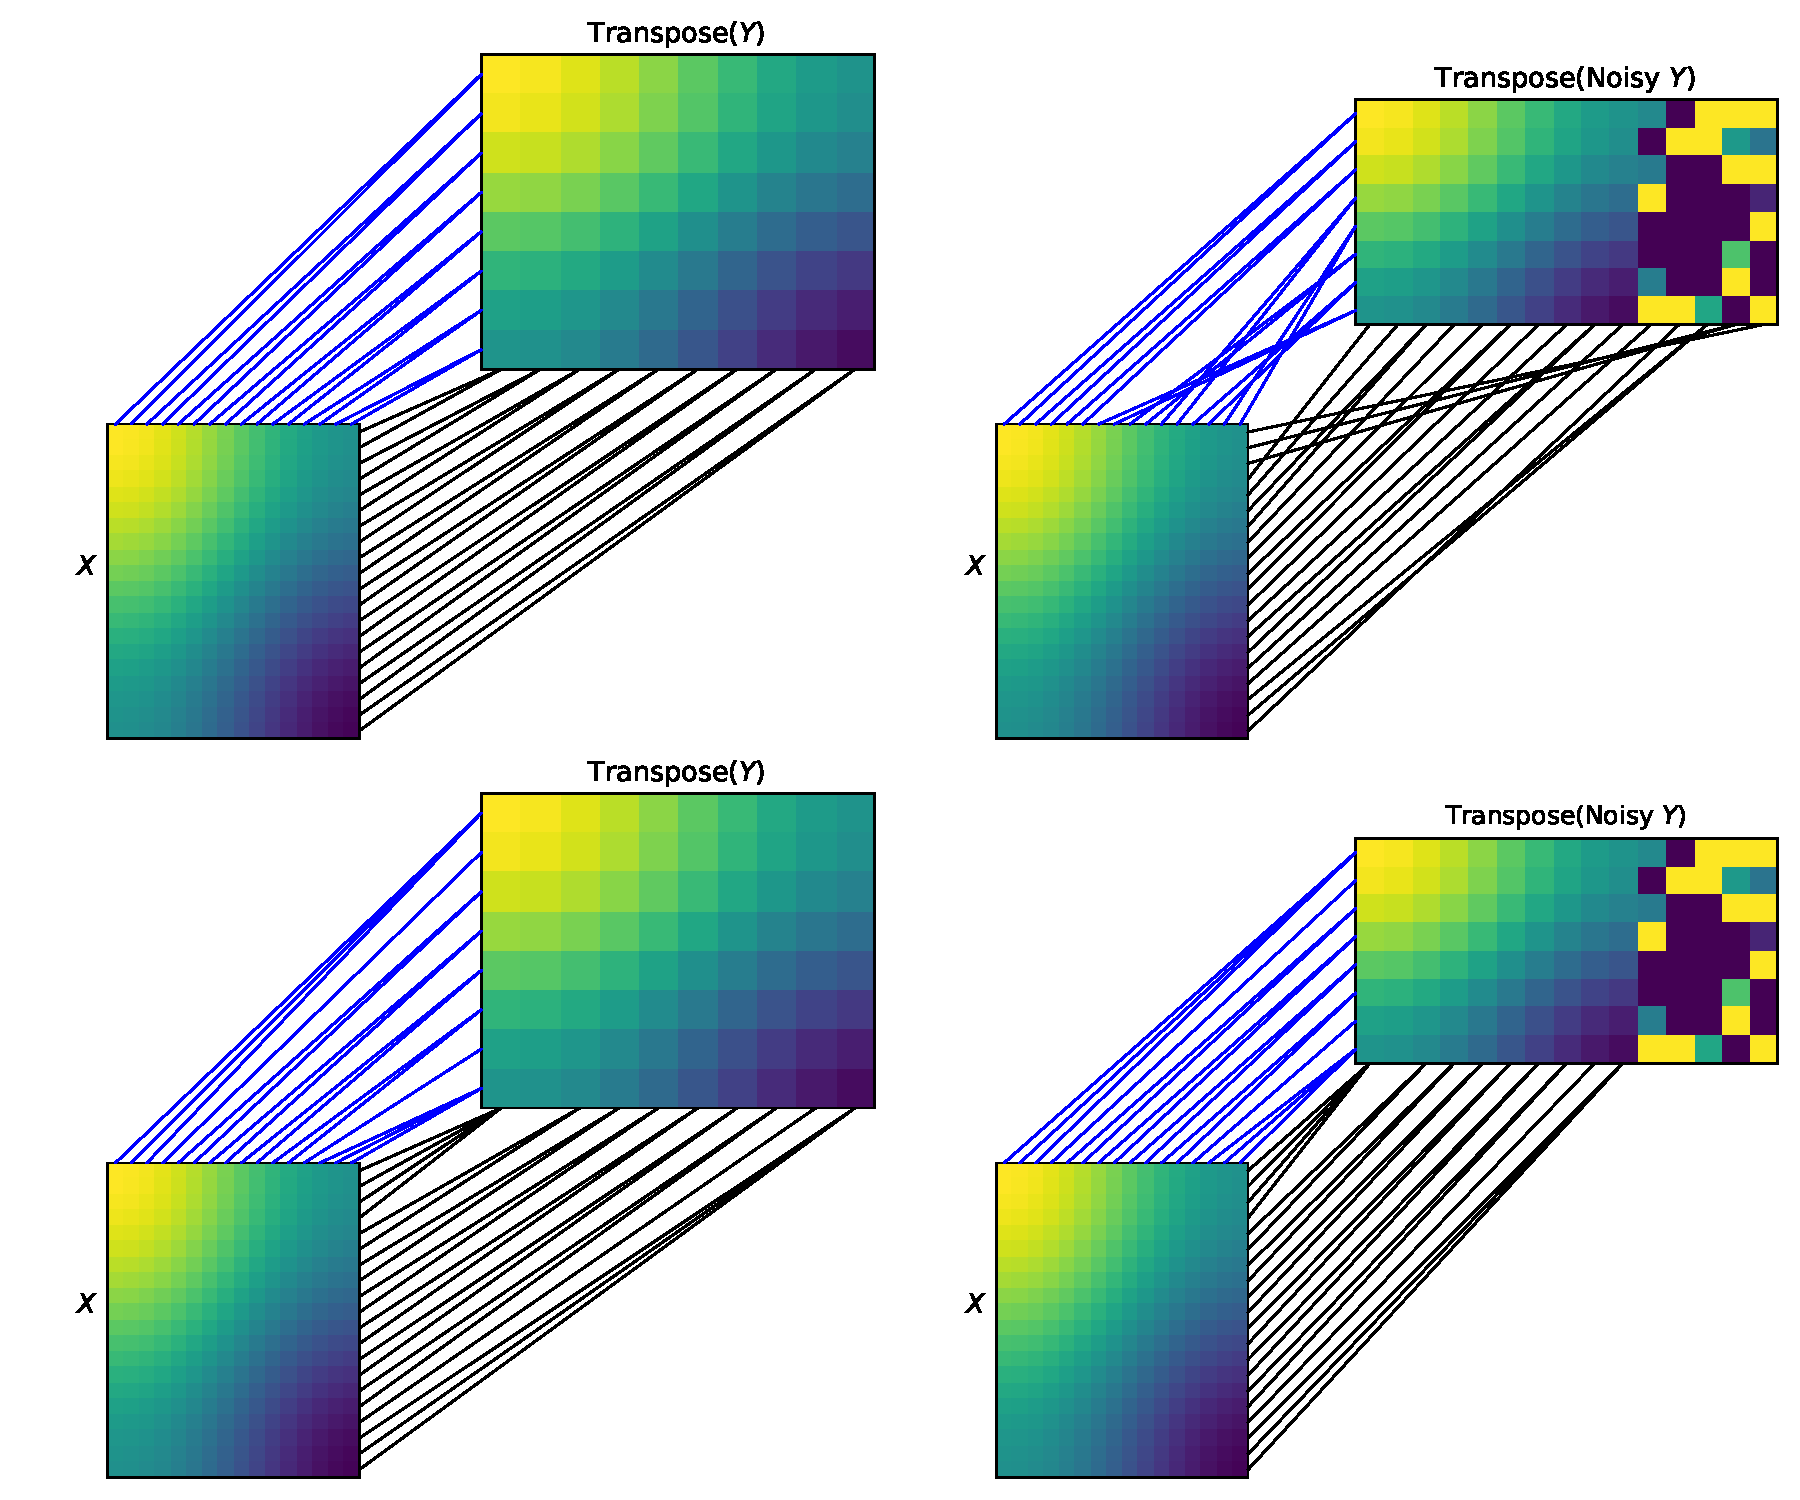
\includegraphics[width=\linewidth, keepaspectratio=true]{OT_new/COOT_plot.pdf}
\end{figure}
\begin{tikzpicture}[remember picture, overlay]
  % we don't want to affect the bounding box if the rectangle is too large
  \begin{pgfinterruptboundingbox}
      % the following coords. may need to be changed to suit your slides
      \fill <1> [fill=white, opacity=0.8] (0,0) rectangle (12, 4.65);
  \end{pgfinterruptboundingbox}
  \node <1> [draw, shape=rectangle, align=right] at (10, 5) {%
      Hello from outliers
  };
\end{tikzpicture}
\end{frame}

%%%%%%%%%%%%%%%%%%%%%%%%%%%%%%%%%%%%
\begin{frame}{Motivation (2)}
  \tiny
  \begin{figure}
    \centering
    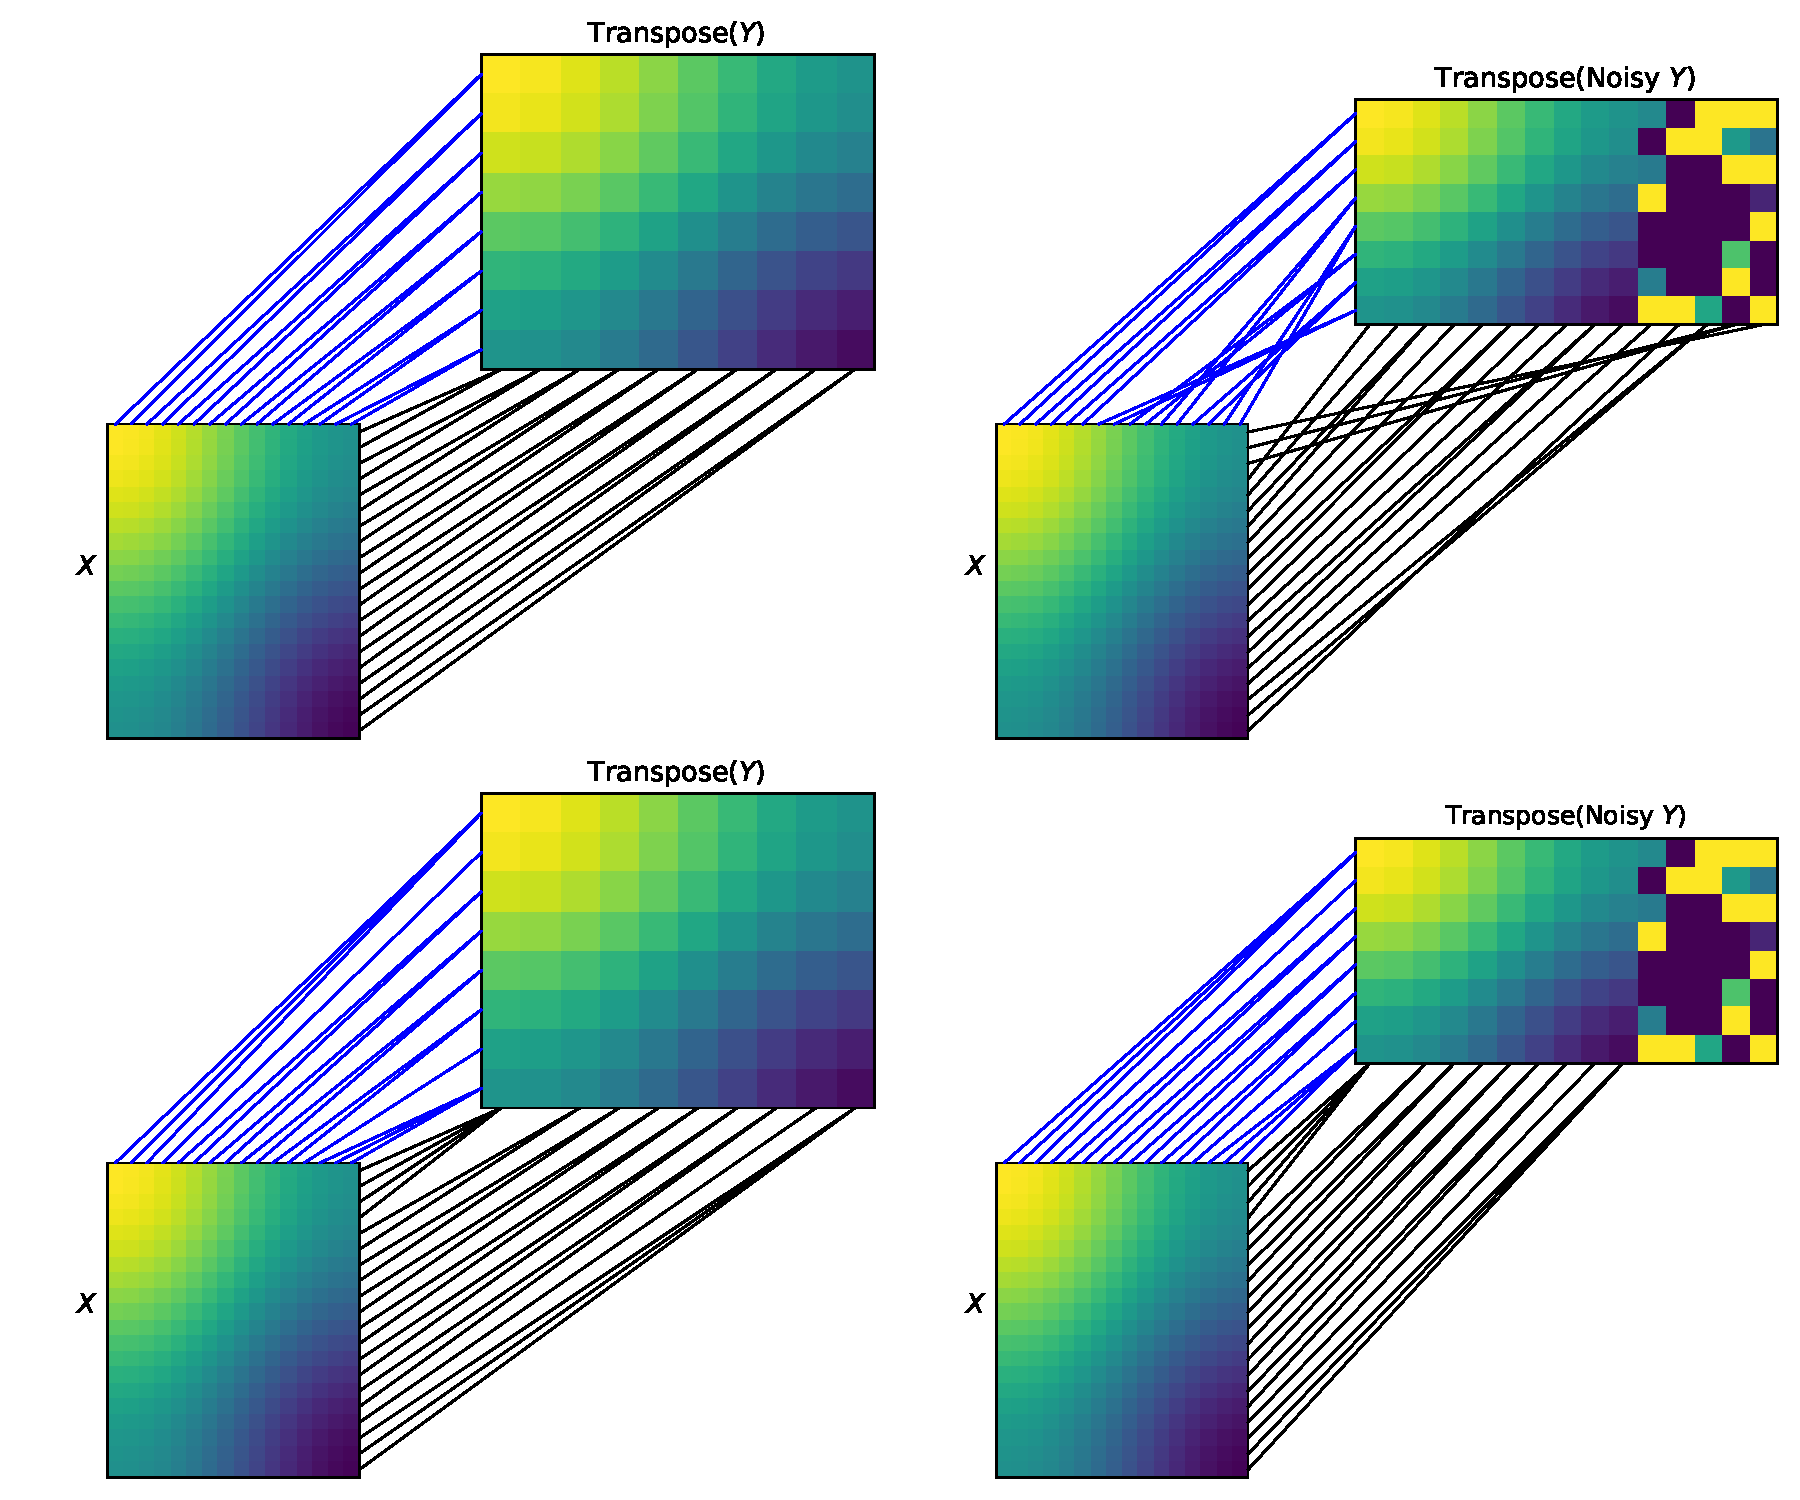
\includegraphics[width=\linewidth, keepaspectratio=true]{OT_new/COOT_plot.pdf}
  \end{figure}
  \begin{tikzpicture}[remember picture, overlay]
    % we don't want to affect the bounding box if the rectangle is too large
    \begin{pgfinterruptboundingbox}
        % the following coords. may need to be changed to suit your slides
        \fill <1> [fill=white, opacity=0.8] (0,4.65) rectangle (12, 8.7);
    \end{pgfinterruptboundingbox}
    \node <1> [draw, shape=rectangle, align=right] at (10.2, 1.6) {%
        Good bye outliers
    };
  \end{tikzpicture}
\end{frame}

%%%%%%%%%%%%%%%%%%%%%%%%%%%%%%%%%%%%
\begin{frame}{Unbalanced CO-Optimal Transport (1)}
\tiny
  \begin{definition}[{\color{blue}{Sample}} - {\color{red}{feature}} space]
      Let ${\color{blue}{(X^s, \mu^s)}}$ and ${\color{red}{(X^f, \mu^f)}}$ be compact measure spaces, where ${\color{blue}{\mu^s \in \cM^+(X^s)}}$ and ${\color{red}{\mu^f \in \cM^+(X^f)}}$. Let $\xi$ be a scalar integrable function in $L^p({\color{blue}{X^s}} \times {\color{red}{X^f}}, {\color{blue}{\mu^s}} \otimes {\color{red}{\mu^f}})$, for some $p \geq 1$. We call
      \begin{itemize}
        \item The triplet  $\cX = \left({\color{blue}{(X^s, \mu^s)}}, {\color{red}{(X^f, \mu^f)}}, \xi \right)$ a \underline{\textit{{\color{blue}{sample}} - {\color{red}{feature}} space}}.

        \item The function $\xi$ an \textit{\underline{interaction}}.
      \end{itemize}
      \end{definition}
  \vspace{-0.2cm}
  \begin{figure}
      \centering
      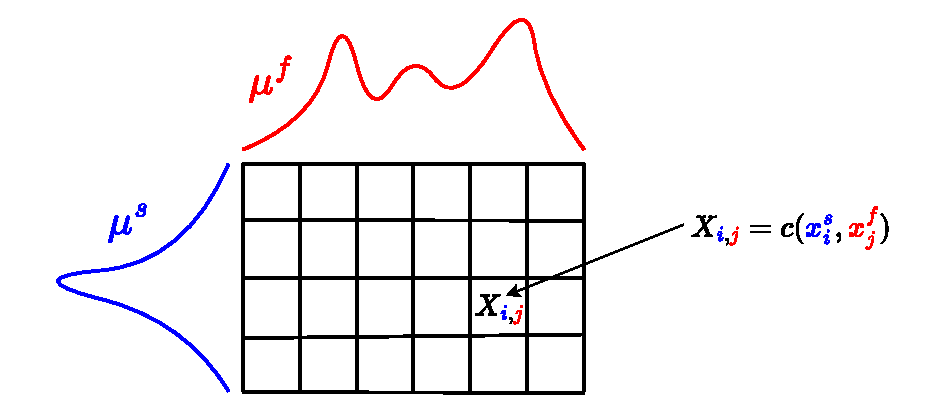
\includegraphics[width=.8\linewidth, keepaspectratio=true]{OT_new/coot_matrix_single.pdf}
  \end{figure}
  \end{frame}

\begin{frame}{Unbalanced CO-Optimal Transport (2)}
\tiny
  \begin{definition}[UCOOT]
      Given $\lambda_1, \lambda_2 >0$ and two s.f. spaces
      $\cX_1 = \left({\color{blue}{(X_1^s, \mu_1^s)}}, {\color{red}{(X_1^f, \mu_1^f)}}, \xi_1 \right)$
      and $\cX_2 = \left({\color{blue}{(X_2^s, \mu_2^s)}}, {\color{red}{(X_2^f, \mu_2^f)}}, \xi_2 \right)$ is defined by:
  \begin{align*}
  \label{eq:ucoot}
      \ucoot_{\lambda}(\cX_1, \cX_2) :=
    \inf_{\substack{{\color{blue}{\pi^s \in \cM^+(X_1^s \times X_2^s)}}
    \\ {\color{red}{\pi^f \in \cM^+(X_1^f \times X_2^f)}}}}
    F(\pis, \pif).
  \end{align*}
  where
  \begin{align*}
      F(\pis, \pif) &= \underbrace{\iint
      |\xi_1({\color{blue}{x_1^s}}, {\color{red}{x_1^f}}) - \xi_2({\color{blue}{x_2^s}}, {\color{red}{x_2^f}})|^p {\color{blue}{\mathrm d\pi^s(x_1^s, x_2^s)}}
      {\color{red}{\mathrm d \pi^f(x_1^f, x_2^f)}}}_{\text{transport cost of {\color{blue}{sample}}-{\color{red}{feature}} pairs}} \\
      &+ \underbrace{\sum_{k=1}^2\lambda_k \text{KL}({\color{blue}{\pi^s_{\# k}}} \otimes {\color{red}{\pi^f_{\# k}}} \vert {\color{blue}{\mu^s_k}} \otimes {\color{red}{\mu^f_k}})}_{\text{mass destruction / creation penalty}}.
  \end{align*}
  \end{definition}
\end{frame}

%%%%%%%%%%%%%%%%%%%%%%%%%%%%%%%%%%%%%%%
\begin{frame}{Why quadratic divergence?}
  \tiny
\begin{enumerate}
  \item Homogeneity.
  \item Existence of solution.
  \item Bilinear relation between minimum and minimizer.
  \begin{align*}
    \ucoot_{\lambda}(\cX_1, \cX_2) =
    \sum_{k=1}^2 \lambda_k m({\color{blue}{\mu_k^s}}) m({\color{red}{\mu_k^f}})
    - (\lambda_1 + \lambda_2) m({\color{blue}{\pi^s_*}}) m({\color{red}{\pi^f_*}}).
  \end{align*}
  \item Restriction to equal-mass solutions: $m({\color{blue}{\pi^s_*}}) = m({\color{red}{\pi^f_*}})$.
  \item Robustness to outlier.
\end{enumerate}

\end{frame}


%%%%%%%%%%%%%%%%%%%%%%%%%
\begin{frame}{Provable robustness of UCOOT (1)}
\tiny
  \begin{definition}
  Consider two \textbf{clean} s.f. spaces
  $\cX_k = \left( {\color{blue}{(X^s_k, \mu^s_k)}}, {\color{red}{(X^f_k, \mu^f_k)}}, \xi_k \right)$,
  for $k = 1, 2$.
  \begin{enumerate}
      \item \textbf{Noisy} s.f. space: $\widetilde{\cX_1} = \left( {\color{blue}{(X^s_1 \cup O^s, \widetilde{\mu}^s_1)}}, {\color{red}{(X^f_1 \cup O^f, \widetilde{\mu}^f_1)}}, \xi_1 \right)$, where
      \begin{itemize}
        \tiny
          \item {\color{blue}{\textbf{Noisy}  distribution on sample space: $\widetilde{\mu}^s_1 = \alpha_s \mu^s_1 + (1-\alpha_s) \varepsilon^s$, where $\alpha_s \in [0,1], \varepsilon^s \in \cM^+(O^s)$.}}
          \item {\color{red}{\textbf{Noisy}  distribution on feature space: $\widetilde{\mu}^f_1 = \alpha_f \mu^f_1 + (1-\alpha_f) \varepsilon^f$, where $\alpha_f \in [0,1], \varepsilon^f \in \cM^+(O^f)$.}}
      \end{itemize}

      \item Minimal cost: $\Delta_{0} := \min_{\substack{
        {\color{blue}{x_1^s \in O^s}}, {\color{red}{x_1^f \in O^f}} \\
        {\color{blue}{x_2^s \in X_2^s}}, {\color{red}{x_2^f \in X_2^f}}}}\quad \left| \xi_1({\color{blue}{x_1^s}}, {\color{red}{x_1^f}}) - \xi_2({\color{blue}{x_2^s}}, {\color{red}{x_2^f}}) \right|^p$.

    \item Maximal cost: $\Delta_{\infty} := \max_{
    \substack{
    {\color{blue}{x_1^s \in X_1^s \cup O^s}}, {\color{red}{x_1^f \in X_1^f \cup O^f}} \\
    {\color{blue}{x_2^s \in X_2^s}}, {\color{red}{x_2^f \in X_2^f}}
    }} \quad \left| \xi_1({\color{blue}{x_1^s}}, {\color{red}{x_1^f}}) - \xi_2({\color{blue}{x_2^s}}, {\color{red}{x_2^f}}) \right|^p$.
  \end{enumerate}
  $\implies$ Both costs can explode if the outliers are too impactful.
  \end{definition}
\end{frame}

\begin{frame}{Provable robustness of UCOOT (2)}
\tiny
\begin{proposition}
  \begin{enumerate}
    \item COOT is sensitive to outliers
    \begin{equation*}
        \coot(\widetilde{\cX_1}, \cX_2) \geq (1 - {\color{blue}{\alpha_s}})(1 - {\color{red}{\alpha_f}})\Delta_0.
    \end{equation*}

    \item Denote
    \begin{itemize}
      \tiny
      \item $\delta = 2(\lambda_1 + \lambda_2)(1 - {\color{blue}{\alpha_s}} {\color{red}{\alpha_f}})$.

      \item $M= m(\pis) = m(\pif)$: mass of OT plans between clean data.

      \item $K = M + \frac{1}{M}\ucoot_{\lambda}(\cX_1, \cX_2) + \delta$.
    \end{itemize}
    Then
    \begin{equation*} %\label{eq:ucoot-robust}
    \begin{split}
      \underbrace{\ucoot_{\lambda}(\widetilde{\cX_1}, \cX_2)}_{\text{"noisy divergence"}}
      &\leq {\color{blue}{\alpha_s}} {\color{red}{\alpha_f}}
      \underbrace{\ucoot_{\lambda}(\cX_1, \cX_2)}_{\text{"clean divergence"}}
      + \underbrace{\delta M \left[ 1 -
      \exp \left( {- \frac{\Delta_{\infty}(1+M) + K}{\delta M}} \right) \right]}_{\text{saturates quickly if } \Delta_{\infty} \to \infty}.
    \end{split}
    \end{equation*}
  \end{enumerate}
\end{proposition}
\end{frame}

%%%%%%%%%%%%%%%%%%%%%%%%%%%%%%%%%
\begin{frame}{Illustration on MNIST images}
\tiny
\begin{figure}
    \centering
    \includegraphics[trim={0.5cm 4.cm 1.5cm 2.4cm}, clip, width=1.\linewidth, keepaspectratio=true]{SIMPAS/mnist-ucoot-rebuttal.pdf}
    \caption*{Example illustrating and interpreting the {\color{red}{feature alignment $\pi^f$}} learned by UCOOT and its robustness to outliers.}
\end{figure}
\end{frame}

%%%%%%%%%%%%%%%%%%%%%%%%%%%%%%%%%
\begin{frame}{Illustration on MNIST images}
\tiny
\begin{figure}
      \centering
      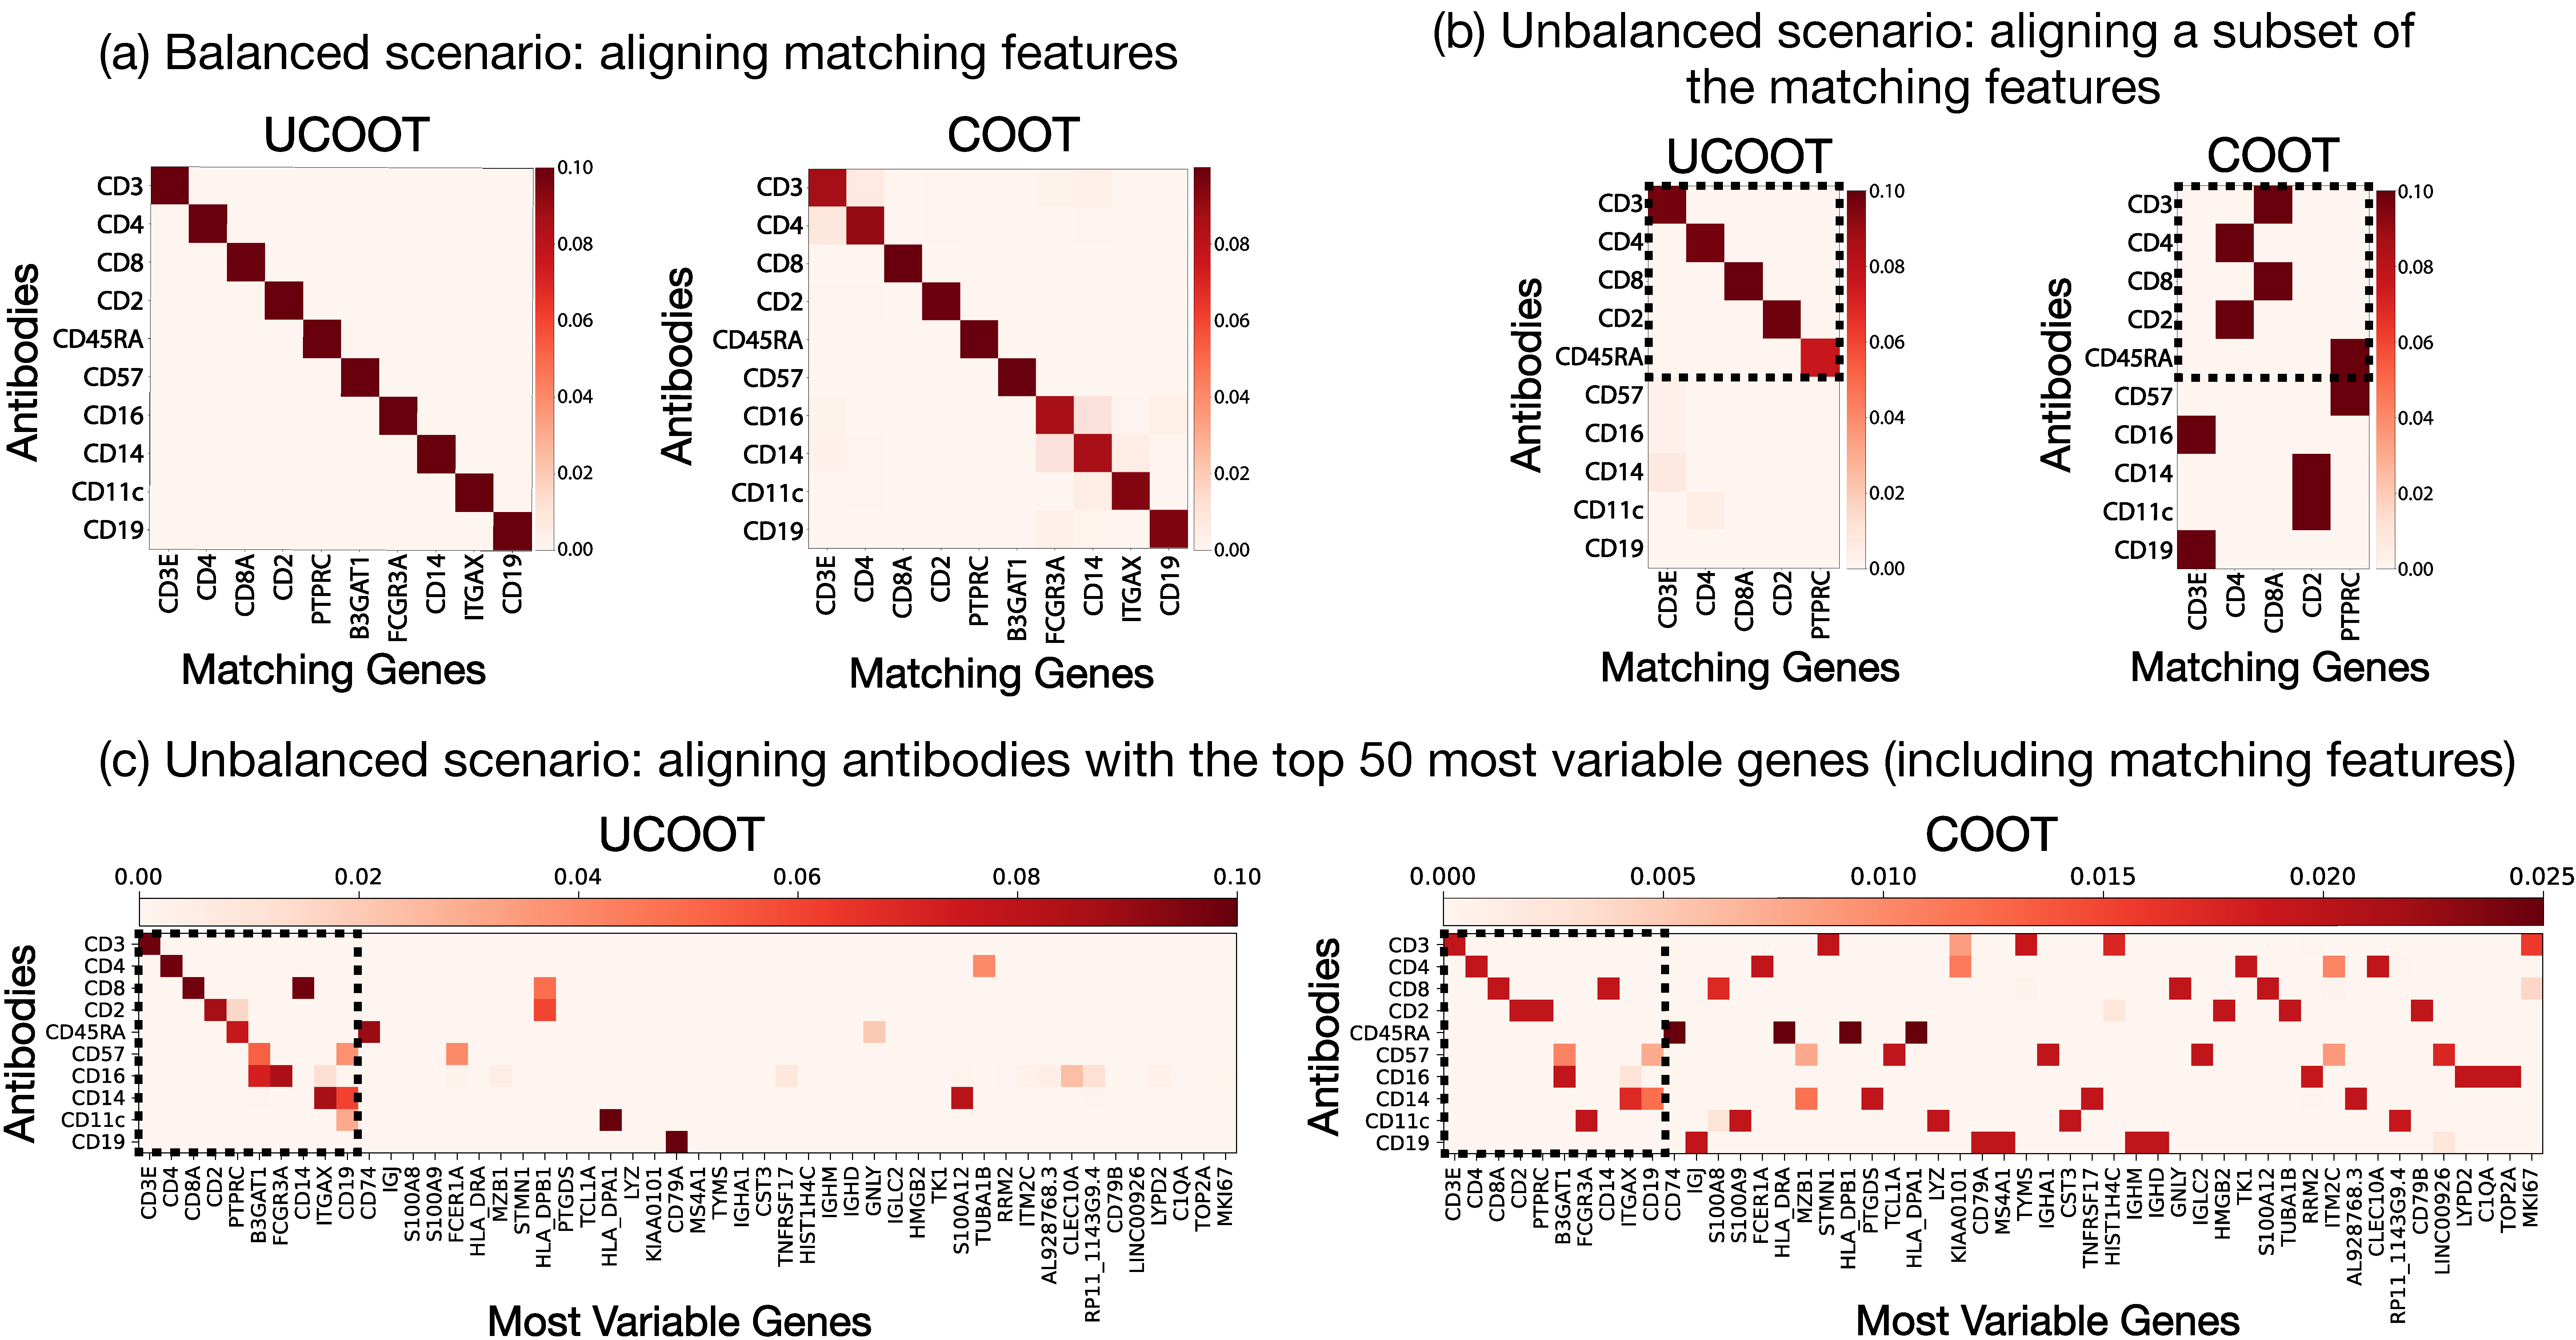
\includegraphics[width=1.\linewidth, keepaspectratio=true]{OT_new/genes-alignments.pdf}
      \caption*{Example illustrating and interpreting the {\color{red}{feature alignment $\pi^f$}} learned by UCOOT and its robustness to outliers.}
  \end{figure}
  \end{frame}

%%%% Contribution on FUGW
\section{Fused Unbalanced Gromov-Wasserstein}

%%%%%%%%%%%%%%%%%%%%%%%%%%%%%%%%%%%%%%%%%%%%
\begin{frame}{Motivation}
\tiny

\end{frame}

%%%%%%%%%%%%%%%%%%%%%%%%%%%%%%%%%%%%%%%%%%%%
\begin{frame}{Formulation}
\tiny
\begin{block}{Definition}
\begin{align*}
  \inf_{P \in \bbR^{m \times n}_{\geq 0}} \quad
  &(1 - \alpha) \sum_{i,j,k,l} | D^s_{ik} - D^t_{jl}|^2 P_{ij} P_{kl}
  + \alpha \sum_{i,j} || F^s_i - F^t_j||_2^2 P_{ij} \\
  &+ \lambda \left[ \kl(P_{\# 1} \otimes P_{\# 1} \vert w^s \otimes w^s)
  + \kl(P_{\# 2} \otimes P_{\# 2} \vert w^t \otimes w^t) \right]
\end{align*}
\end{block}
\begin{figure}
  \centering
  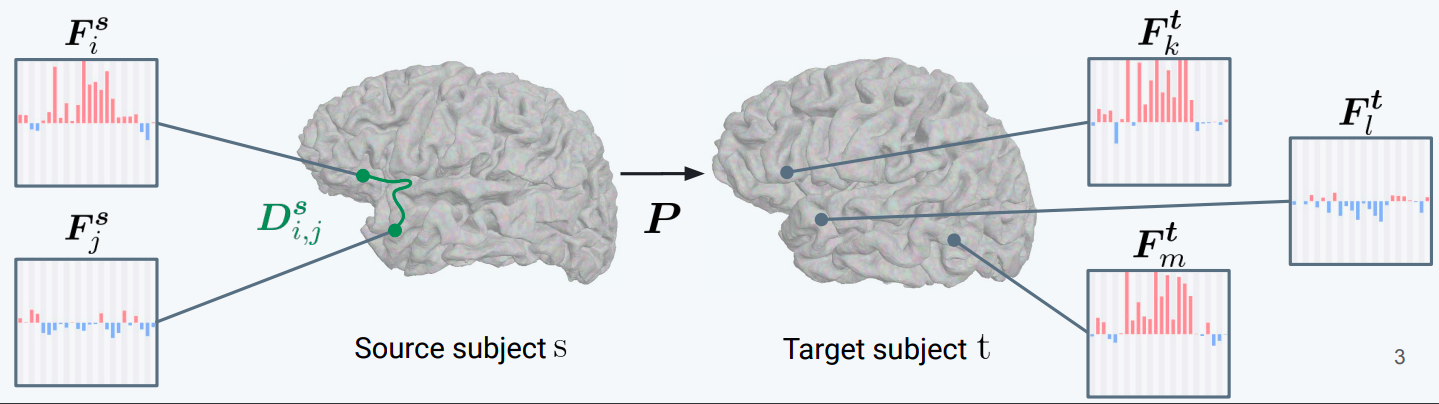
\includegraphics[width=1.\linewidth, keepaspectratio=true]{OT_new/fugw.png}
  \caption*{Neuroscientific interpretation}
\end{figure}
\end{frame}

%%%%%%%%%%%%%%%%%%%%%%%%%%%%%%%%%%%%%%%%%%%%%%%%%%%%%%%%%%%%%%%%%%%%%%
%%%%%%%%%%%%%%%%%%%%%%%%%%%%%%%%%%%%%%%%%%%%%%%%%%%%%%%%%%%%%%%%%%%%%%
%%%%%%%%%%%%%%%%%%%%%%%%%%%%%%%%%%%%%%%%%%%%%%%%%%%%%%%%%%%%%%%%%%%%%%
%%%% Contribution on AGW
\section{Augmented Gromov-Wasserstein}

%%%%%%%%%%%%%%%%%%%%%%%%%%%%%%%%%%%%%%
\begin{frame}{Motivation}
%%%%%%%%%%%%%%%%%%%%%%%%%%%%%%%%%
\tiny
\begin{enumerate}
  \item Isometries are useful for across-space comparison.
  \item All isometries are created equal, but some are more equal than others.
  \item GW induces all isometries but none for COOT.
\end{enumerate}
\begin{figure}
    \centering
    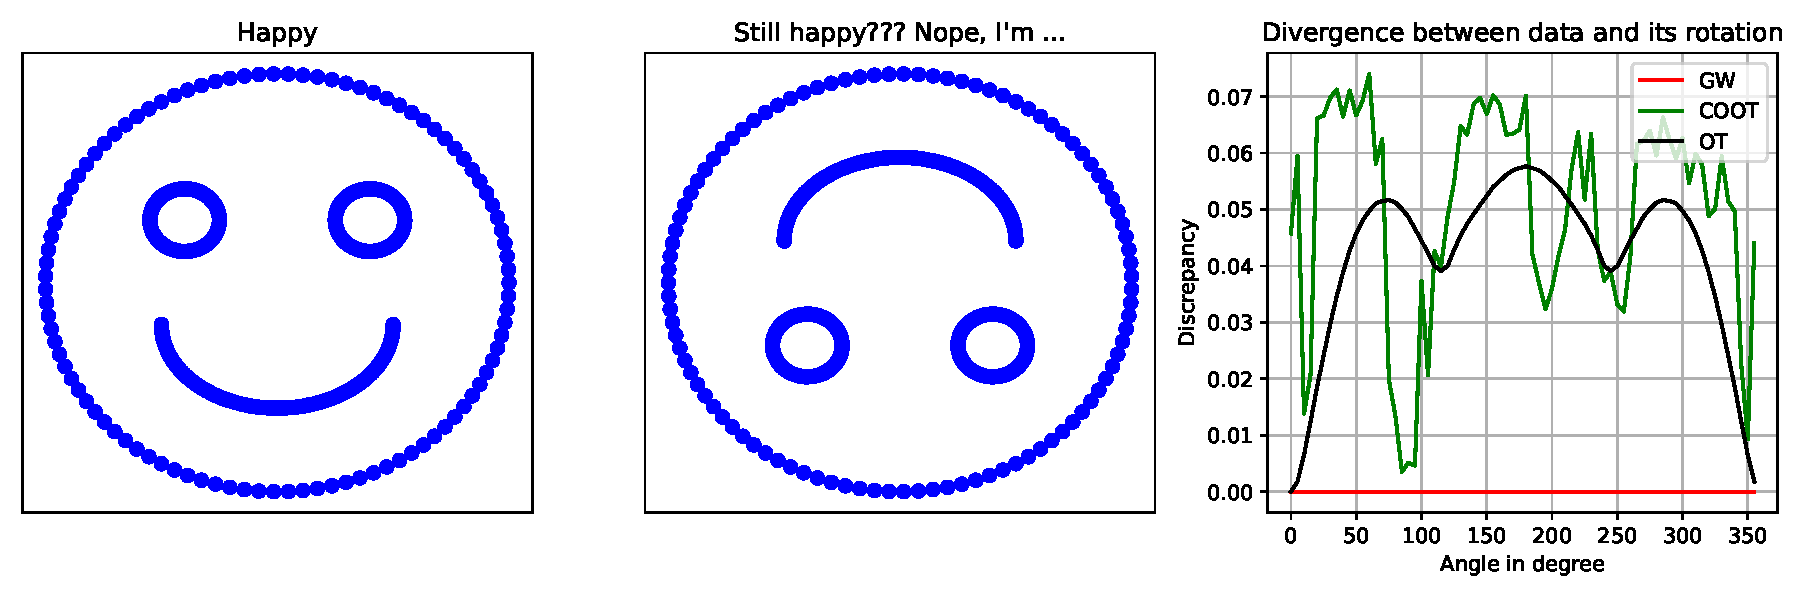
\includegraphics[width=1.\linewidth, keepaspectratio=true]{OT_new/div_vs_angle.pdf}
\end{figure}
\end{frame}

%%%%%%%%%%%%%%%%%%%%%%%%%%%%%%%%%%%%%%
\begin{frame}{Formulation}
\tiny
\begin{block}{Definition}
  Given two weighted matrices $\cX_1 = (X_1, \mssrc, \mfsrc)$
  and $\cX_2 = (X_2, \mstg, \mftg)$, for $0\leq \alpha \leq 1$,
  \begin{align*}
    \label{eq:scootr}
    \agw_{\alpha}(\cX_1, \cX_2) &:=
    \min_{\substack{\pis \in U(\mssrc,\mstg) \\ \pif \in U(\mfsrc,\mftg)}}
    L_{\alpha}(\pis, \pif),
  \end{align*}
  where $L_{\alpha}(\pis, \pif) =
  \alpha \; \langle L(D_X,D_Y)\otimes \pis, \pis \rangle
  + (1-\alpha) \; \langle L(X,Y) \otimes \pis, \pif \rangle$.
  % \begin{align*}
  %   L_{\alpha}(\pis, \pif) &=
  %   \alpha \; \langle L(D_X,D_Y)\otimes \pis, \pis \rangle
  %   + (1-\alpha) \; \langle L(X,Y) \otimes \pis, \pif \rangle.
  % \end{align*}
\end{block}
\begin{minipage}[t]{0.6\linewidth}
  \begin{itemize}
    \item Interpolating between GW and COOT.
    \item Satisfying relaxed triangle inequality.
  \end{itemize}
  \end{minipage}%
  \hfill%
  \hspace{-6cm}
  \begin{minipage}[t]{0.5\linewidth}
    \vspace{-0.2cm}
  \begin{figure}
    \centering
    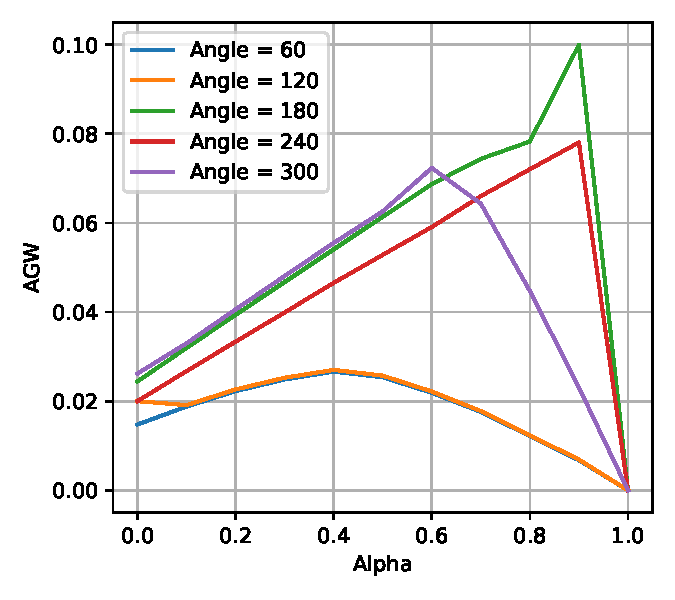
\includegraphics[width=0.85\linewidth, keepaspectratio=true]{OT_new/agw_alpha.pdf}
  \end{figure}
  \end{minipage}

\end{frame}

%%%%%%%%%%%%%%%%%%%%%%%%%%%%%%%%%%%%%%
\begin{frame}{Isometries}
\tiny
\vspace{-0.2cm}
\begin{itemize}
  \item Only finitely many isometries such that $\agw_{\alpha}(\cX_1, \cX_2) = 0$.
\end{itemize}
\begin{assumption}
  \label{assumption:1}
Given an input matrix $X \in \bbR^{n \times d}$, assume
\begin{enumerate}
  \item[(A1)] $n \geq d$: Low-dimensional setting.
  \item[(A2)] $X$ is full rank: Easily met by preprocessing.
  \item[(A3)] $X$ has $d$ distinct singular values. Fact:
  set of Hermitian matrices with repeated eigenvalues has zero Lebesgue measure.
\end{enumerate}
\end{assumption}
\begin{proposition}
  Given two weighted matrices $\cX_1 = (X_1, \mssrc, \mfsrc)$
  and $\cX_2 = (X_2, \mstg, \mftg)$,
  \begin{enumerate}
      \item[$(\Rightarrow)$] If $\mssrc = \mstg$ and
      $X_2$ is obtained by permuting columns of $X_1$ via
      the permutation $\sigma_c$ (so $\mftg = (\sigma_c)_{\#} \mfsrc$),
      then $\agw_{\alpha}(\cX_1, \cX_2) = 0$.
      \item[$(\Leftarrow)$] Suppose $X_1$ satisfies A1-A3. For any $0 < \alpha < 1$,
      if $\agw_{\alpha}(\cX_1, \cX_2) = 0$,
      then there exist a symmetric orthogonal matrix $O \in \mathcal O_d$
      and a permutation matrix $P \in \mathcal P_d$ such that $X_2 = X_1 OP$.
  \end{enumerate}
\end{proposition}
\end{frame}

%%%%%%%%%%%%%%%%%%%%%%%%%%%%%%%%%
\begin{frame}{Experiments}
\tiny
\begin{figure}
  \centering
  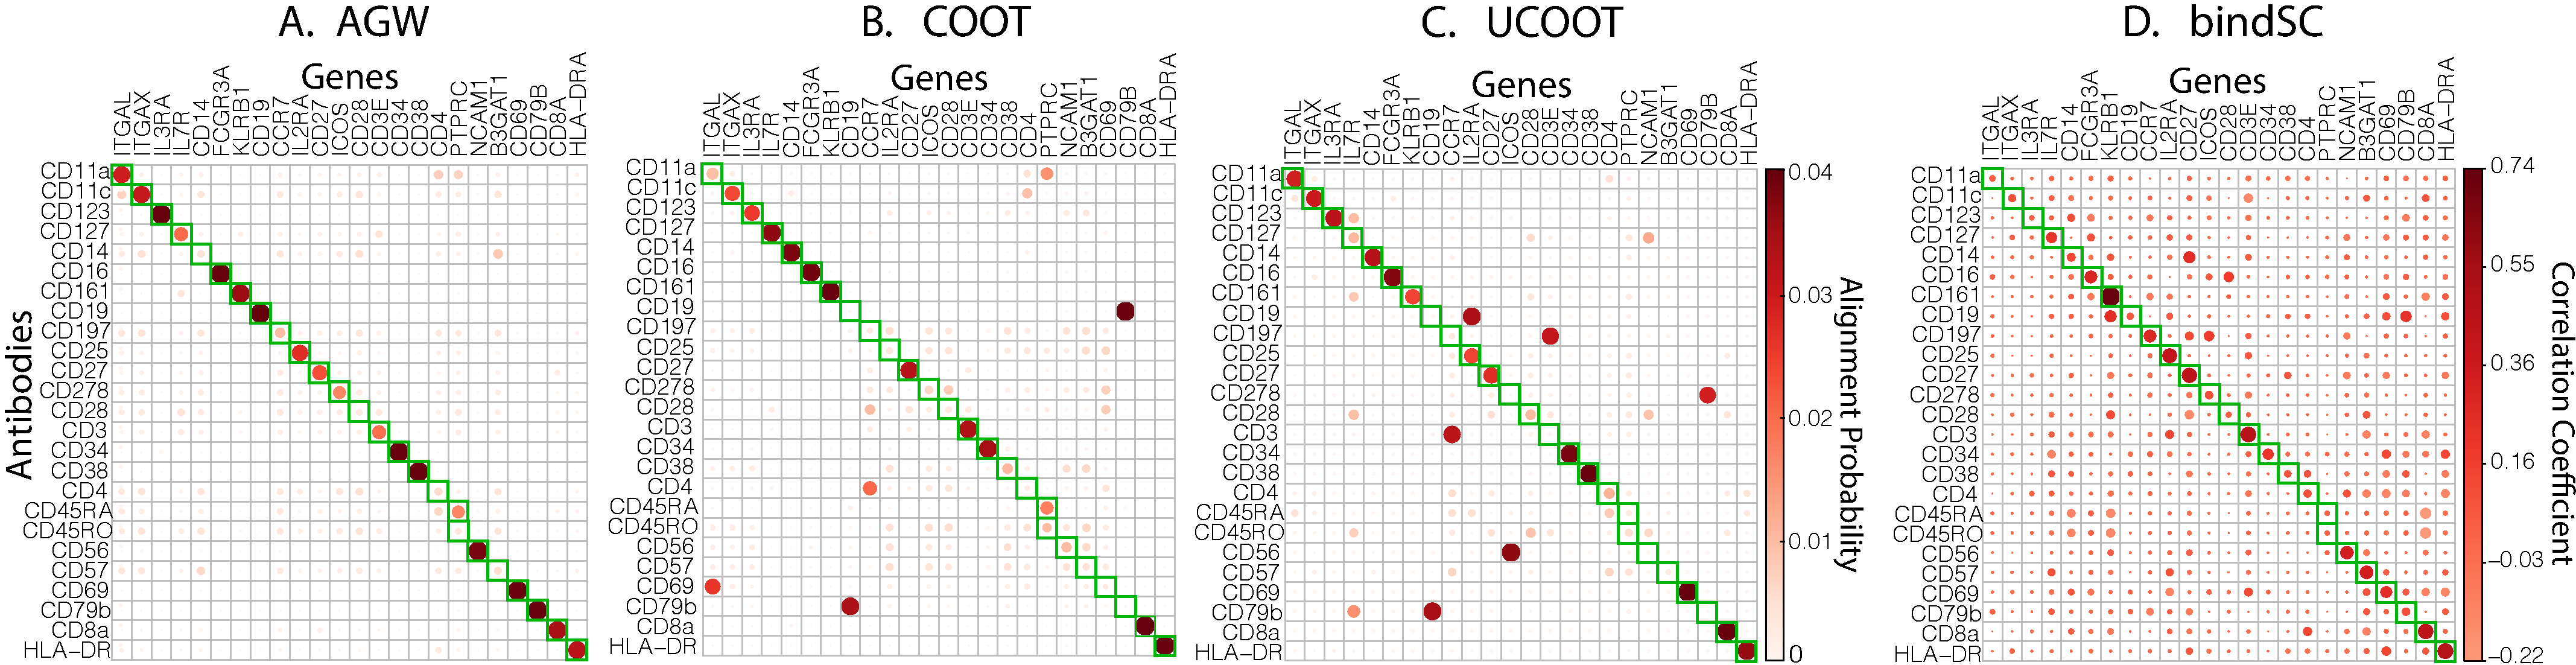
\includegraphics[width=1.\linewidth, keepaspectratio=true]{OT_new/cite_fgcoot_final.pdf}
  \caption*{Neuroscientific interpretation}
\end{figure}
\end{frame}

\section{Conclusion and Perspective}
%%%%%%%%%%%%%%%%%%%%%%%%%%%%%%%%%%
\begin{frame}{Conclusion and Perspective}
\tiny
\begin{itemize}
  \item Conclusion
  \begin{enumerate}
    \item
  \end{enumerate}

  \item Perspectives
  \begin{enumerate}
    \tiny
    \item In general, statisical aspects of unbalanced across-space divergences
    are still little understood.
    \item Practical consideration: UGW, FUGW, UCOOT rely on BCD
    $\Rightarrow$ More efficient UOT solvers.
  \end{enumerate}
\end{itemize}
\end{frame}

%%%%%%%%%%%%%%%%%%%%%%%%%%%%%%%%%%
\begin{frame}
  \centering \Large
  \textbf{{Thank you for your attention}}
\end{frame}

%%%%%%%%%%%%%%%%%%%%%%%%%%%%%%
\section*{References}
%%%%%%%%%%%%%%%%%%%%%%%%%%%%%%%%%%%%%%%
\begin{frame}[allowframebreaks]{References}
\tiny
\printbibliography
\end{frame}

\begin{frame}
  Why bilinear relation.

\end{frame}

\end{document}